\documentclass[12pt,letterpaper]{article}
\usepackage{graphicx,textcomp}
\usepackage{natbib}
\usepackage{setspace}
\usepackage{fullpage}
\usepackage{color}
\usepackage[reqno]{amsmath}
\usepackage{amsthm}
\usepackage{fancyvrb}
\usepackage{amssymb,enumerate}
\usepackage[all]{xy}
\usepackage{endnotes}
\usepackage{lscape}
\newtheorem{com}{Comment}
\usepackage{float}
\usepackage{hyperref}
\newtheorem{lem} {Lemma}
\newtheorem{prop}{Proposition}
\newtheorem{thm}{Theorem}
\newtheorem{defn}{Definition}
\newtheorem{cor}{Corollary}
\newtheorem{obs}{Observation}
\usepackage[compact]{titlesec}
\usepackage{dcolumn}
\usepackage{tikz}
\usetikzlibrary{arrows}
\usepackage{multirow}
\usepackage{subcaption}
\usepackage{xcolor}
\newcolumntype{.}{D{.}{.}{-1}}
\newcolumntype{d}[1]{D{.}{.}{#1}}
\definecolor{light-gray}{gray}{0.65}
\usepackage{url}
\usepackage{listings}
\usepackage{color}
\usepackage{mathtools} 
\usepackage{amsmath}
\usepackage{amssymb}
\usepackage{color,soul}

\definecolor{codegreen}{rgb}{0,0.6,0}
\definecolor{codegray}{rgb}{0.5,0.5,0.5}
\definecolor{codepurple}{rgb}{0.58,0,0.82}
\definecolor{backcolour}{rgb}{0.95,0.95,0.92}

\lstdefinestyle{mystyle}{
	backgroundcolor=\color{backcolour},   
	commentstyle=\color{codegreen},
	keywordstyle=\color{magenta},
	numberstyle=\tiny\color{codegray},
	stringstyle=\color{codepurple},
	basicstyle=\footnotesize,
	breakatwhitespace=false,         
	breaklines=true,                 
	captionpos=b,                    
	keepspaces=true,                 
	numbers=left,                    
	numbersep=5pt,                  
	showspaces=false,                
	showstringspaces=false,
	showtabs=false,                  
	tabsize=2
}
\lstset{style=mystyle}
\newcommand{\Sref}[1]{Section~\ref{#1}}

\title{Submission for Problem Set 1}
\date{Duc Minh, VU \\
TCD StudentID: 22996761 / UCD StudentID: 19211157}
\author{Applied Stats/Quant Methods 1}

\begin{document}
\maketitle
\section*{Question 1: Education}
\noindent Data will first be loaded or in this case manually constructed: 

\lstinputlisting[language=R, firstline=15, lastline=15]{Problem Set 1_R_Code.R}

\begin{enumerate} 
	\item \textbf{Calculation of 90\% confidence interval for student IQ}
	\begin{enumerate}
		\item \textit{Step 1: Calculation of the sample mean:}\\
		$\bullet$ Calculation of sample mean manually:
			\lstinputlisting[language=R, firstline=20, lastline=20]{Problem Set 1_R_Code.R}
		The sample mean for the IQ score calculated manually is 98.44. \\
		$\bullet$ Calculation of sample mean using R:
			\lstinputlisting[language=R, firstline=22, lastline=22]{Problem Set 1_R_Code.R}
		The sample mean for the IQ score calculated using R is also 98.44. \\
		$\bullet$ Using R to double-check if the manual score is the same as the R-calculated score:
			\lstinputlisting[language=R, firstline=24, lastline=24]{Problem Set 1_R_Code.R}
		\begin{verbatim}
			[1] TRUE
		\end{verbatim}
		R output confirms that the manually caculated mean score is equal to/the same as the R-calculated mean score.
		\item \textit{Step 2: Calculation of the sample variance and standard deviation:}\\
		$\bullet$ Manual calculation:
			\lstinputlisting[language=R, firstline=28, lastline=29]{Problem Set 1_R_Code.R}
		The manually caclulated value for the sample variance is 171.42333, and for the standard deviation is 13.0929. \\
		$\bullet$ Calculation using R:
			\lstinputlisting[language=R, firstline=31, lastline=32]{Problem Set 1_R_Code.R}
		The R-caclulated value for the sample variance and standard deviation is also 171.42333, and 13.0929 respectively.\\
		$\bullet$ Using R to double-check the results between the manual and the R calculation:
			\lstinputlisting[language=R, firstline=24, lastline=24]{Problem Set 1_R_Code.R}
		\begin{verbatim}
			[1] TRUE
		\end{verbatim}
		R output confirms that the manually caculated score is equal to/the same as the R-calculated score for variance and standard deviation.
		\item \textit{Step 3: Finding the associated t-score :}\\
		Since the number of observation in the dataset is less than 30, t-distribution is more appropriated and will be used.
			\lstinputlisting[language=R, firstline=44, lastline=44]{Problem Set 1_R_Code.R}
		The t-score at 90\% confidence level is 1.71
		\item \textit{Step 4: Caclculating the confidence interval}\\
		The confidence interval will be calculated as:
		\begin{center}
		$\bar{y}$ {\textpm} t-value \texttimes Standard Errors
		\end{center}
		Based on the results from the two previous steps, the ... observations from the IQ test scores are summarized by $\bar{y}$ = 98.44 and \textit{s} = 13.0929. The estimated standard error of the sampling distribution of $\bar{y}$ can be calculated as: 
			$${SE(Standard Errors) = \frac{\textit{s}}{\sqrt{n}}}$$
			\lstinputlisting[language=R, firstline=49, lastline=49]{Problem Set 1_R_Code.R}
		Which gives the result of 2.6186 in R.
			\lstinputlisting[language=R, firstline=53, lastline=55]{Problem Set 1_R_Code.R}
		\begin{verbatim}
			> conf_int_t
			[1]  93.95993 102.92007
		\end{verbatim}
	\end{enumerate} 
	\item \textbf{Hypothesis testing for the average student IQ versus the country average IQ score}
	\begin{enumerate}
		\item \textit{Assumptions} \\
		It will be assumed that the school counselor's sample is randomly selected and normally distributed. The IQ scores itself are quantitative data.
		
		\item \textit{Generation of hypotheses}\\
		Let {\textmu} be the population mean for the school's average IQ score. Since the school counselor is interested in whether her school's average score is HIGHER than the country's average score of 100, the alternative hypothesis will be one-sided:
 				$${\textbf{H\textsubscript{1} \textgreater 100 }}$$
 		And thus the null hypothesis will be:
 				$${\textbf{H\textsubscript{0} $\le$ 100 }}$$
 				
		\item \textit{Calculation of test statistic}\\
		Based on the value of the sample mean and estimated standard error from the previous part, the test statistic is
			$${t = \frac{\bar{y} - \mu}{\textit{se}}}$$
			\lstinputlisting[language=R, firstline=64, lastline=64]{Problem Set 1_R_Code.R}
		which gives the result of -0.5957.
		
		\item \textit{Calculation of P-value}\\
		For n = 25, the degree freedom is n - 1 = 24. Hence, the probability (P-value) of a t-score above the observed t-score or the right-tail probability abolve -0.5967 is:
			 \lstinputlisting[language=R, firstline=68, lastline=68]{Problem Set 1_R_Code.R}
		which gives the result P = 0.7215.
		
		\item \textit{Conclusion}\\
		With sample mean $\bar{y}$ = 98.44, the P-value is 0.7215 which is very large. If \textmu = 100, it would not be unusual to observe $\bar{y}$ = 98.44. Since P-value is larger than $\alpha$ (0.7215 \textgreater 0.05), we fail to reject the null hypothesis H\textsubscript{0}. Students in the counselor's chool doesn't have higher average IQ scores than students among all the schools in the country. Check P.199 in textbook
		
	\end{enumerate}
\end{enumerate} 

\section*{Question 2: Political Economy}
\graphicspath{ {C:/Users/Admin/Documents/GitHub/StatsI_Fall2022/problemSets/PS01/Assignment Submission/Graph} }
\begin{enumerate} 
	\item \textbf{The relationships between Y, X1, X2 and X3} \\
	Figure 1 contains the scatterplots for all of the relationships between Y, X1, X2 and X3. The next section will go into detail the relationship for each pair of the variables.\\
		\begin{figure}[h!]\centering
			\caption{\footnotesize Scatterplots of all the relationships between Y, X1, X2 and X3 .}
			\label{fig:plot_1}
			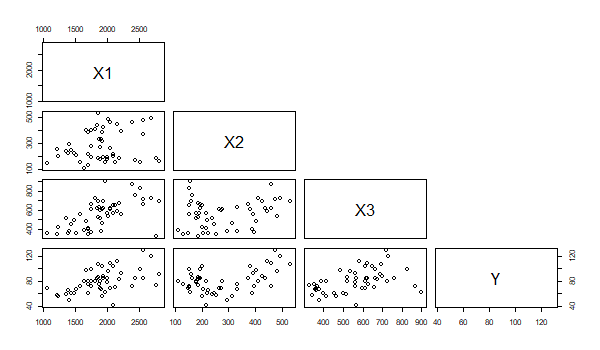
\includegraphics[width=.85\textwidth]{1.corr_plot_all_vars.png}
		\end{figure}
	
	\begin{enumerate}
		\item The relationship between Y and X1 \\
		Figure 2 displays the relationship between Per capita expenditure on housing assistance (Y) and Per capita income (X1). From the graph, there seems to be a positive relationship between the two varaibles, as Y increases and X1 increases
		\begin{figure}[h!]\centering
			\caption{\footnotesize Scatterplot between Y and X1.}
			\label{fig:plot_1}
			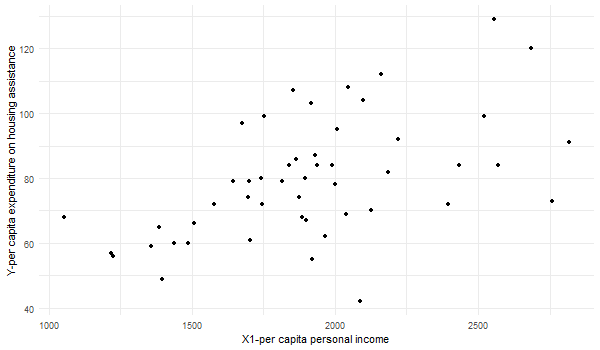
\includegraphics[width=.85\textwidth]{1.1.corr_plot_Y_and_X1.png}
		\end{figure}
		
		\item The relationship between Y and X2 \\
		\begin{figure}[h!]\centering
			\caption{\footnotesize Scatterplot between Y and X2.}
			\label{fig:plot_1}
			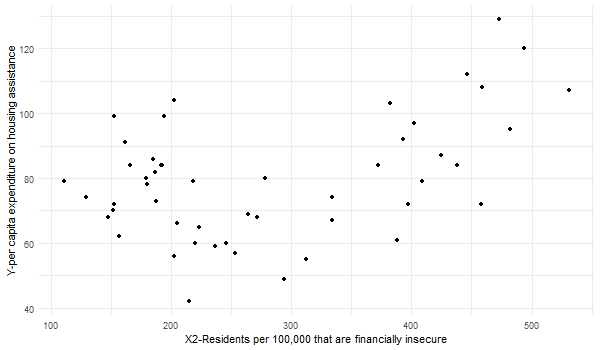
\includegraphics[width=.85\textwidth]{1.2.corr_plot_Y_and_X2.png}
		\end{figure}
	
		\item The relationship between Y and X3 \\
		\begin{figure}[h!]\centering
			\caption{\footnotesize Scatterplot between Y and X3.}
			\label{fig:plot_1}
			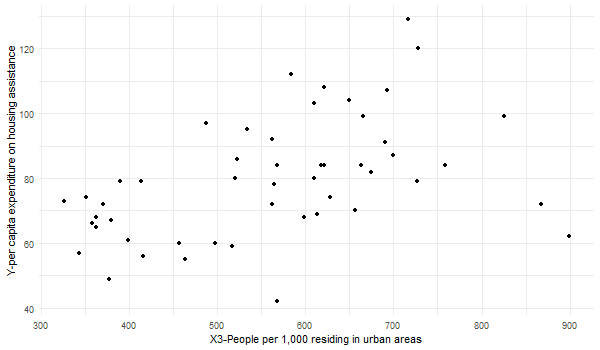
\includegraphics[width=.85\textwidth]{1.3.corr_plot_Y_and_X3.png}
		\end{figure}
		
		\item The relationship between X1 and X2 \\
		\begin{figure}[h!]\centering
			\caption{\footnotesize Scatterplot between X1 and X2.}
			\label{fig:plot_1}
			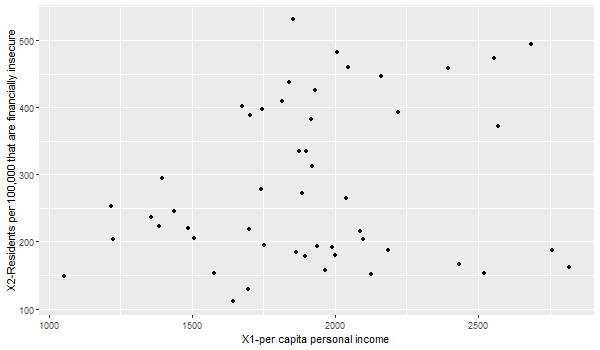
\includegraphics[width=.85\textwidth]{1.4.corr_plot_X1_and_X2.png}
		\end{figure}
	
		\item The relationship between X1 and X3 \\
		\begin{figure}[h!]\centering
			\caption{\footnotesize Scatterplot between X1 and X3.}
			\label{fig:plot_1}
			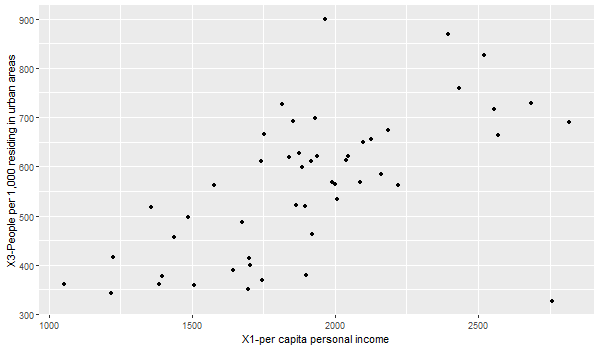
\includegraphics[width=.85\textwidth]{1.5.corr_plot_X1_and_X3.png}
		\end{figure}

	\end{enumerate} 
\end{enumerate} 

\end{document}